\documentclass[11pt]{article}
\usepackage[utf8]{inputenc}
\usepackage[T1]{fontenc}
\usepackage{amsmath}
\usepackage{amssymb} % Needed for \eth
\usepackage{graphicx}
\usepackage{geometry}
\usepackage{tikz}
\usepackage{pgfplots} % For plots
\usepackage{ulem}     % For underline, using normalem to avoid messing with \emph
\usepackage{booktabs} % For tables if needed
\usepackage{tcolorbox} % For boxing equations if needed
\usepackage{braket}    % For QM state notation if needed

\geometry{a4paper, margin=1in}
\usetikzlibrary{positioning, arrows.meta, shapes.geometric, patterns, calc} % Added calc library
\pgfplotsset{compat=1.18} % Use a recent PGFPlots version

% Custom commands (optional)
\newcommand{\avg}[1]{\overline{#1}}
\newcommand{\prob}[1]{P(#1)}
\newcommand{\ProbDens}[1]{\mathcal{P}(#1)} % Using script P for density
\newcommand{\vect}[1]{\vec{#1}}
\newcommand{\dd}[1]{\mathrm{d}#1} % Differential d
\newcommand{\pderiv}[2]{\frac{\partial #1}{\partial #2}}
\newcommand{\deriv}[2]{\frac{\mathrm{d} #1}{\mathrm{d} #2}}
\newcommand{\muState}{\mu\text{-state}} % Microstate
\newcommand{\OmegaE}{\Omega(E)}
\newcommand{\omegaE}{\omega(E)}
\newcommand{\PhiE}{\Phi(E)}
\newcommand{\deltaE}{\delta E}
\newcommand{\ethbar}{\text{\it{đ}}} % \eth symbol for inexact differential
\newcommand{\kb}{k_B} % Boltzmann constant
\newcommand{\gasR}{R} % Ideal gas constant
\newcommand{\partfn}{Z} % Partition function symbol
\newcommand{\grandpartfn}{\mathcal{Z}} % Grand partition function symbol (using \mathcal{Z})
\newcommand{\eps}{\epsilon}

\title{Physics 415 - Lecture 28: Quantum Statistics}
\date{April 2, 2025}
\author{} % Author not specified

\begin{document}

\maketitle
\thispagestyle{empty}

\section*{Summary}

\begin{itemize}
    \item Canonical Ensemble (CE): Fixed $T, N, V$. $P_r = e^{-\beta E_r} / \partfn$, $\partfn = \sum_r e^{-\beta E_r}$ ($\beta=1/T$). $F = -T \ln \partfn$.
    \item Grand Canonical Ensemble (GCE): Fixed $T, \mu, V$. $P_r = e^{-\beta(E_r - \mu N_r)} / \grandpartfn$, $\grandpartfn = \sum_r e^{-\beta(E_r - \mu N_r)}$. $\Phi = -T \ln \grandpartfn$. Relation $\grandpartfn = \sum_N e^{\beta \mu N} Z_N$. Mean particle number $\avg{N} = -(\partial \Phi / \partial \mu)_{T,V}$.
\end{itemize}

\section*{Quantum Ideal Gases (Identical Particles)}

Energy of a state is $E = n_1 \eps_1 + n_2 \eps_2 + \dots = \sum_r n_r \eps_r$, where $\eps_r$ are single-particle energy levels and $n_r$ are occupation numbers.
The allowed occupation numbers depend on the particle statistics:
\[ n_r = \begin{cases} 0, 1, 2, \dots & \text{Bose-Einstein (BE) Statistics (Bosons)} \\ 0, 1 & \text{Fermi-Dirac (FD) Statistics (Fermions)} \end{cases} \]
Total particle number constraint: $\sum_r n_r = N$.

\subsection*{Ground State (T=0)}
Consider the drastic difference between BE and FD statistics in the quantum ground state (lowest total energy state). Let single-particle energies be ordered $\eps_1 < \eps_2 < \eps_3 < \dots$.

\textbf{BE Ground State:} To minimize total energy $E = \sum n_r \eps_r$ subject to $\sum n_r = N$, all $N$ particles occupy the lowest single-particle state $\eps_1$.
\begin{itemize}
    \item Occupation numbers: $n_r = N \delta_{r,1}$.
    \item Ground state energy: $E_{BE}^{(0)} = N \eps_1$.
\end{itemize}

\begin{center}
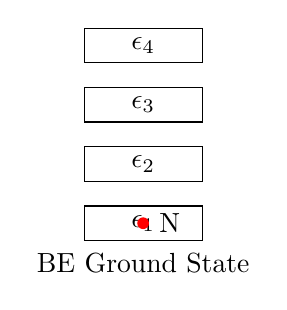
\begin{tikzpicture}[level/.style={draw, minimum width=1.5cm, minimum height=0.15cm}]
    \node[level] (e1) at (0,0) {$\eps_1$};
    \node[level] (e2) [above=0.3cm of e1] {$\eps_2$};
    \node[level] (e3) [above=0.3cm of e2] {$\eps_3$};
    \node[level] (e4) [above=0.3cm of e3] {$\eps_4$};
    \node at (e1.center) [fill=red, circle, inner sep=1.5pt, label=right:N] {};
    \node at (0, -0.5) {BE Ground State};
\end{tikzpicture}
\end{center}

\textbf{FD Ground State:} Due to the Pauli exclusion principle ($n_r=0$ or $1$), particles must fill the lowest available energy states, one particle per state, until all $N$ particles are placed.
\begin{itemize}
    \item Occupation numbers: $n_r = 1$ for $r=1, \dots, N$; $n_r=0$ for $r>N$.
    \item Ground state energy: $E_{FD}^{(0)} = \eps_1 + \eps_2 + \dots + \eps_N$.
\end{itemize}
Note that $E_{FD}^{(0)} > E_{BE}^{(0)}$ (for $N>1$). The highest occupied energy level $\eps_N$ is called the Fermi energy $E_F$.

\begin{center}
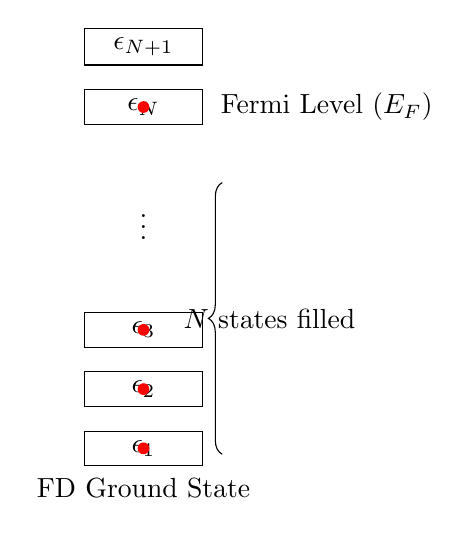
\begin{tikzpicture}[level/.style={draw, minimum width=1.5cm, minimum height=0.15cm}]
    \node[level] (e1) at (0,0) {$\eps_1$};
    \node[level] (e2) [above=0.3cm of e1] {$\eps_2$};
    \node[level] (e3) [above=0.3cm of e2] {$\eps_3$};
    \node[level] (eN) [above=0.8cm of e3, draw=none] {$\vdots$};
    \node[level] (eN1) [above=0.8cm of eN] {$\eps_N$};
    \node[level] (eN2) [above=0.3cm of eN1] {$\eps_{N+1}$};

    \node at (e1.center) [fill=red, circle, inner sep=1.5pt] {};
    \node at (e2.center) [fill=red, circle, inner sep=1.5pt] {};
    \node at (e3.center) [fill=red, circle, inner sep=1.5pt] {};
    \node at (eN1.center) [fill=red, circle, inner sep=1.5pt] {};

    \draw [decorate, decoration={brace, amplitude=5pt}, xshift=1cm] (0,-0.075) -- (0,3.375) node [midway, xshift=0.6cm] {$N$ states filled};
    \node at (eN1.east) [right=0.1cm] {Fermi Level ($E_F$)};
    \node at (0, -0.5) {FD Ground State};
\end{tikzpicture}
\end{center}

\subsection*{Mean Occupation Numbers ($\overline{n}_r$)}

When $T>0$, particles will be "thermally excited" to higher energy states. This leads to a change in the mean occupation numbers $\overline{n}_r$.
BE: $\overline{n}_1 < N$, $\overline{n}_{r>1} > 0$.
FD: $\overline{n}_{r \le N} < 1$, $\overline{n}_{r > N} > 0$.

Calculating $\overline{n}_r$ in the Canonical Ensemble (CE):
\[ \overline{n}_r = \sum_{\{n_1, n_2, \dots\}}' P_{\{n_k\}} n_r \]
where $P_{\{n_k\}} = e^{-\beta \sum_k n_k \eps_k} / Z_N$ and the sum $\sum'$ is restricted by $\sum_k n_k = N$.
It can be shown that:
\[ \overline{n}_r = -\frac{1}{\beta} \pderiv{(\ln Z_N)}{\eps_r} = T \pderiv{(\ln Z_N)}{\eps_r} \]
(Similar to how $\avg{E} = -\partial(\ln Z)/\partial \beta$).
However, calculating $Z_N$ with the constraint $\sum n_r = N$ is challenging.

\subsection*{Using the Grand Canonical Ensemble (GCE)}

The calculation becomes much simpler in the GCE because the constraint $\sum n_r = N$ is lifted (N fluctuates, fixed by reservoir $\mu$). The sum over states $\{n_1, n_2, \dots\}$ becomes unrestricted (subject only to $n_r \ge 0$ for BE or $n_r \in \{0,1\}$ for FD).
The grand partition function is:
\[ \grandpartfn = \sum_{\{n_1, n_2, \dots\}} e^{-\beta \sum_k (\eps_k - \mu) n_k} \]
Because the sum in the exponent is over independent states $k$, and the sum over $\{n_k\}$ is unrestricted, the sum factorizes:
\[ \grandpartfn = \left( \sum_{n_1} e^{-\beta(\eps_1-\mu)n_1} \right) \times \left( \sum_{n_2} e^{-\beta(\eps_2-\mu)n_2} \right) \times \dots = \prod_r \left( \sum_{n_r} e^{-\beta(\eps_r-\mu)n_r} \right) \]
The sum $\sum_{n_r}$ depends on the statistics:

\textbf{BE Statistics ($n_r = 0, 1, 2, \dots$):}
The sum is a geometric series: $\sum_{k=0}^\infty x^k = 1/(1-x)$, with $x = e^{-\beta(\eps_r-\mu)}$.
The series converges only if $|x|<1$, which requires $e^{-\beta(\eps_r-\mu)} < 1 \implies \eps_r - \mu > 0$, or $\mu < \eps_r$ for all $r$. Thus, the chemical potential $\mu$ must be less than the minimum single-particle energy $\eps_{min}$.
\[ \sum_{n_r=0}^{\infty} e^{-\beta(\eps_r-\mu)n_r} = \frac{1}{1 - e^{-\beta(\eps_r-\mu)}} \]
\[ \implies \grandpartfn_{BE} = \prod_r \frac{1}{1 - e^{-\beta(\eps_r-\mu)}} \]
The grand potential $\Phi = -T \ln \grandpartfn$:
\[ \Phi_{BE} = T \sum_r \ln(1 - e^{-\beta(\eps_r-\mu)}) \]

\textbf{FD Statistics ($n_r = 0, 1$):}
The sum has only two terms:
\[ \sum_{n_r=0}^{1} e^{-\beta(\eps_r-\mu)n_r} = e^0 + e^{-\beta(\eps_r-\mu)} = 1 + e^{-\beta(\eps_r-\mu)} \]
\[ \implies \grandpartfn_{FD} = \prod_r (1 + e^{-\beta(\eps_r-\mu)}) \]
The grand potential:
\[ \Phi_{FD} = -T \sum_r \ln(1 + e^{-\beta(\eps_r-\mu)}) \]

We can write a single expression for $\Phi$ covering both cases:
\[ \Phi = \pm T \sum_r \ln(1 \mp e^{-\beta(\eps_r-\mu)}) \]
(Upper sign: BE, Lower sign: FD).

\subsection*{Mean Occupation Numbers $\overline{n}_r$ in GCE}

The average occupation number of a single-particle state $r$ is:
\[ \overline{n}_r = \sum_{\{n_k\}} P_{\{n_k\}} n_r = \frac{1}{\grandpartfn} \sum_{\{n_k\}} n_r e^{-\beta \sum_k (\eps_k-\mu)n_k} \]
Because $\grandpartfn$ factorizes, $\grandpartfn = \grandpartfn_r \times \prod_{k \neq r} \grandpartfn_k$, where $\grandpartfn_r = \sum_{n_r} e^{-\beta(\eps_r-\mu)n_r}$.
The average becomes:
\[ \overline{n}_r = \frac{\sum_{n_r} n_r e^{-\beta(\eps_r-\mu)n_r}}{\sum_{n_r} e^{-\beta(\eps_r-\mu)n_r}} \]
(All terms from $k \neq r$ cancel between numerator and denominator).
This average can be calculated using the logarithm trick:
\[ \overline{n}_r = -\frac{1}{\beta} \pderiv{}{\eps_r} \ln\left( \sum_{n_r} e^{-\beta(\eps_r-\mu)n_r} \right) \]

\textbf{BE Case:} $\ln(\sum \dots) = -\ln(1 - e^{-\beta(\eps_r-\mu)})$.
\[ \overline{n}_r = -\frac{1}{\beta} \pderiv{}{\eps_r} [-\ln(1 - e^{-\beta(\eps_r-\mu)})] = \frac{1}{\beta} \frac{1}{1-e^{-\beta(\dots)}} [-e^{-\beta(\dots)}(-\beta)] \]
\[ \overline{n}_r = \frac{e^{-\beta(\eps_r-\mu)}}{1 - e^{-\beta(\eps_r-\mu)}} = \frac{1}{e^{\beta(\eps_r-\mu)} - 1} \]
This is the \textbf{Bose-Einstein distribution} function, giving the mean number of bosons in state $r$.

\textbf{FD Case:} $\ln(\sum \dots) = \ln(1 + e^{-\beta(\eps_r-\mu)})$.
\[ \overline{n}_r = -\frac{1}{\beta} \pderiv{}{\eps_r} [\ln(1 + e^{-\beta(\eps_r-\mu)})] = -\frac{1}{\beta} \frac{1}{1+e^{-\beta(\dots)}} [e^{-\beta(\dots)}(-\beta)] \]
\[ \overline{n}_r = \frac{e^{-\beta(\eps_r-\mu)}}{1 + e^{-\beta(\eps_r-\mu)}} = \frac{1}{e^{\beta(\eps_r-\mu)} + 1} \]
This is the \textbf{Fermi-Dirac distribution} function, giving the mean number of fermions in state $r$.

(Note: In both cases, $\overline{n}_r$ could also be obtained from $\overline{n}_r = -\partial \Phi / \partial \eps_r$, holding $T, \mu$ constant).

The mean total particle number is $\avg{N}$:
\[ \avg{N} = -\left( \pderiv{\Phi}{\mu} \right)_{T,V} \]
Let's check this yields $\sum_r \overline{n}_r$:
\[ -\pderiv{\Phi}{\mu} = -\pderiv{}{\mu} \left[ \pm T \sum_r \ln(1 \mp e^{-\beta(\eps_r-\mu)}) \right] \]
\[ = \mp T \sum_r \frac{1}{1 \mp e^{-\beta(\dots)}} [\mp e^{-\beta(\dots)} (-\beta)(-\pderiv{\mu}{\mu})] \]
\[ = \mp T \sum_r \frac{\mp \beta e^{-\beta(\eps_r-\mu)}}{1 \mp e^{-\beta(\eps_r-\mu)}} = T \beta \sum_r \frac{e^{-\beta(\eps_r-\mu)}}{1 \mp e^{-\beta(\eps_r-\mu)}} \]
\[ = \sum_r \frac{1}{e^{\beta(\eps_r-\mu)} \mp 1} = \sum_r \overline{n}_r \]
So $\avg{N} = \sum_r \overline{n}_r$, an obvious result. If we view $N$ as fixed, this equation becomes an implicit relation that determines $\mu = \mu(T, N, V)$.

\subsection*{Special Case: Photon Statistics}

There are certain bosonic particles whose total number is not fixed (not conserved), e.g., photons (quantized oscillations of E\&M field) which can be emitted and absorbed by atoms, or phonons/magnons (elementary excitations in solids).
These are treated using Bose-Einstein statistics but without the constraint $\sum n_r = N$. This is equivalent to using the GCE formalism with chemical potential $\mu=0$.

The mean occupation number becomes (Planck distribution):
\[ \overline{n}_r = \frac{1}{e^{\beta \eps_r} - 1} \]
Alternatively, calculate $Z$ in CE but with unrestricted sum over $\{n_r\}$:
$Z = \sum_{\{n_1, n_2, \dots\}} e^{-\beta (n_1\eps_1 + n_2\eps_2 + \dots)}$. Factorizes:
$Z = (\sum_{n_1=0}^\infty e^{-\beta\eps_1 n_1}) (\sum_{n_2=0}^\infty e^{-\beta\eps_2 n_2}) \dots = \prod_r \frac{1}{1-e^{-\beta\eps_r}}$.
This matches $\grandpartfn_{BE}$ with $\mu=0$.

\end{document}